%%%%%%%%%%%%%%%%%%%%%%%%%%%%%%%%%%%%%%%%%
% Beamer Presentation
% LaTeX Template
% Version 1.0 (10/11/12)
%
% This template has been downloaded from:
% http://www.LaTeXTemplates.com
%
% License:
% CC BY-NC-SA 3.0 (http://creativecommons.org/licenses/by-nc-sa/3.0/)
%
%%%%%%%%%%%%%%%%%%%%%%%%%%%%%%%%%%%%%%%%%

%----------------------------------------------------------------------------------------
%	PACKAGES AND THEMES
%----------------------------------------------------------------------------------------

%\documentclass{beamer}
\documentclass[aspectratio=169]{beamer}

\usepackage[utf8x]{inputenc}
\usepackage{url}
\usepackage{eqnarray}
\usepackage{graphicx}
%\usepackage[spanish]{babel}
\usepackage{mathtools}
\usepackage{color}
\DeclarePairedDelimiter{\ceil}{\lceil}{\rceil}

\mode<presentation> {

% The Beamer class comes with a number of default slide themes
% which change the colors and layouts of slides. Below this is a list
% of all the themes, uncomment each in turn to see what they look like.

%\usetheme{default}
%\usetheme{AnnArbor}
%\usetheme{Antibes}
%\usetheme{Bergen}
%\usetheme{Berkeley}
%\usetheme{Berlin}
%\usetheme{Boadilla}
%\usetheme{CambridgeUS}
%\usetheme{Copenhagen}
\usetheme{Darmstadt}
%\usetheme{Dresden}
%\usetheme{Frankfurt}
%\usetheme{Goettingen}
%\usetheme{Hannover}
%\usetheme{Ilmenau}
%\usetheme{JuanLesPins}
%\usetheme{Luebeck}
%\usetheme{Madrid}
%\usetheme{Malmoe}
%\usetheme{Marburg}
%\usetheme{Montpellier}
%\usetheme{PaloAlto}
%\usetheme{Pittsburgh}
%\usetheme{Rochester}
%\usetheme{Singapore}
%\usetheme{Szeged}
%\usetheme{Warsaw}

% As well as themes, the Beamer class has a number of color themes
% for any slide theme. Uncomment each of these in turn to see how it
% changes the colors of your current slide theme.

%\usecolortheme{albatross}
\usecolortheme{beaver}
%\usecolortheme{beetle}
%\usecolortheme{crane}
\usecolortheme{dolphin}
%\usecolortheme{dove}
%\usecolortheme{fly}
%\usecolortheme{lily}
%\usecolortheme{orchid}
%\usecolortheme{rose}
%\usecolortheme{seagull}
%\usecolortheme{seahorse}
%\usecolortheme{whale}
%\usecolortheme{wolverine}

%\setbeamertemplate{footline} % To remove the footer line in all slides uncomment this line
%\setbeamertemplate{footline}[page number] % To replace the footer line in all slides with a simple slide count uncomment this line

%\setbeamertemplate{navigation symbols}{} % To remove the navigation symbols from the bottom of all slides uncomment this line
}
%\newcommand{\abrcuatrimetre}{sep_dic_2020}
\usepackage{graphicx} % Allows including images
\usepackage{booktabs} % Allows the use of \toprule, \midrule and \bottomrule in tables

%----------------------------------------------------------------------------------------
%	TITLE PAGE
%----------------------------------------------------------------------------------------

\title[SI]{Sistemas Inteligentes} % The short title appears at the bottom of every slide, the full title is only on the title page

\author{Dr. Marco Aurelio Nuño Maganda} % Your name
\institute[UPV] % Your institution as it will appear on the bottom of every slide, may be shorthand to save space
{
Universidad Politecnica de Victoria \\ % Your institution for the title page
Ingenieria en Tecnologias de la Informacion \\ % Your institution for the title page
Cuatrimestre Enero-Abril 2022  \\ % Your institution for the title page
\medskip
\textit{mnunom@upv.edu.mx} % Your email address
}
\date{\today} % Date, can be changed to a custom date

\addtobeamertemplate{navigation symbols}{}{%
    \usebeamerfont{footline}%
    \usebeamercolor[fg]{footline}%
    \hspace{1em}%
    \insertframenumber/\inserttotalframenumber
}
\usepackage{setspace}


\begin{document}

\begin{frame}
\titlepage % Print the title page as the first slide
\end{frame}




%------------------------------------------------
\section{Presentación} 

\begin{frame}

\frametitle{¿Cuales son las credenciales del profesor?}
\begin{itemize}
\item Doctor en Ciencias Computacionales por parte del INAOE (2009).  
\item Profesor de Tiempo Completo de la UPV desde 2009.  
\item Miembro del Sistema Nacional de Investigadores - Nivel Candidado (2014-2016), Nivel I (2020-2022)
\item Asignaturas impartidas en el pasado (Cómputo en Dispositivos Moviles, Graficación por Computadora Avanzada, Lenguajes y Automátas, Sistemas Operativos).
\item Miembro del Nucleo Academico Basico (NAB) de la maestria en Ingeniería de la UPV.
\item 14 tesis dirigidas a nivel maestría.
\end{itemize}


\end{frame}


\section{Clase}

\begin{frame}
\frametitle{Horario de la Clase}


\begin{itemize}
\item Días y horas de clase
\tiny
\begin{spacing}{1.0}
\begin{center}
\begin{tabular}{c|ccccc}
\hline 
          & Lunes       & Martes        & Miércoles   & Jueves & Viernes       \\  \hline 
ITI-27798 & 11:10-12:05 & 11:10 - 12:05 & 9:45-12:05 &  11:10 - 12:05   & 11:10 - 12:05  \\
ITI-27804 & 12:05-13:00 & 12:05-13:00 & 12:05-13:00 &  12:05-13:00      & 12:05-13:55  \\      
\hline
\end{tabular}
\end{center}
\end{spacing}
\normalsize


\item Fechas Importantes:
\begin{itemize}
\item Inicio de Cursos: 3/Enero
\item Fin de Cursos: 19/Abril
\item Dias no hábiles oficiales: 7 de febrero (lunes) y 21 de marzo (lunes), 14 y 15 de abril (jueves y viernes). 
\end{itemize}
\end{itemize}

\end{frame}


\begin{frame}
\begin{itemize}
\frametitle{Plataforma Virtual para el Curso}
\item Nombre de la clase: \textbf{Sistemas Inteligentes - ENE-ABR 2022}
\item Código de clase en Classroom: \textbf{zlz6gxv}
\item Enlace Meet para sesiones no presenciales: \textbf{https://meet.google.com/irs-kvgx-dfr}
\end{itemize}

\end{frame}


\begin{frame}
\frametitle{Reglas basicas}
\begin{itemize}
\item Se recomienda puntualidad y asistencia a las sesiones.
\item Respecto hacia el profesor y hacia sus compañeros y compañeras.  
\item No se permite el ingreso y/o ingestión de \textbf{Alimentos} ni \textbf{Bebidas} de ningún tipo a la clase (ni aún estando en sus hogares). 
\item Cámaras deben encenderse en el momento que se les solicite, además de estar a la vista. 
\end{itemize}
\end{frame}

\begin{frame}
\frametitle{Politica de Pase de Lista}
\begin{itemize}
\item Se pasa lista múltiples veces de manera automática a lo largo de la clase y sin previo aviso.
\item Se recomienda utilizar su cuenta institucional de la universidad, ya que no se autorizará el ingreso de ningún participante externo a la universidad.  
\item Para justificar una inasistencia, es necesario cumplir con los siguientes pasos:
\begin{itemize}	 
\item Agendar una asesoría de la clase mediante el SIITA, verificar que el profesor marque la asesoría como realizada y confirmar la asesoría.
\item En cualquier espacio al final de una clase, solicitar al profesor su registro de justificación.
\item  \textbf{NO ES NECESARIO ENVIAR correo electrónico al profesor -- }
\end{itemize}
%\item Elementos a adjuntar para justificación: receta, carta de defunción, comprobante de tramite, etc, etc.
\end{itemize}
\end{frame}

\begin{frame}
\frametitle{Asistencias minimas para aprobar asignatura}
\begin{itemize}
\item Total de clases al cuatrimestre: 5 * 15 semanas, total 75 - cuatro dias no hábiles, 71 clases 
\item Al NO alcanzar un 80\% de asistencia, (60 asistencias, 15 faltas), el estudiante pierde su derecho de ser EVALUADO
\end{itemize}


\end{frame}


\begin{frame}
\frametitle{Puntos Extra por Asistencia}
\begin{itemize}
\item Total de clases al cuatrimestre: 5 * 15 semanas, total 75 - cuatro dias no hábiles, 71 clases 
\item Al lograr un 95\% de asistencia (71 asistencias, 4 faltas), el estudiante adquiere el derecho a 10 puntos extras sobre su calificacion final, siempre y cuando la calificacion final sea mayor a 70. Adémas, si el estudiante cae en la situacion ``recursamiento de ultima unidad'', se permitirá siempre y cuando cumpla con este mismo porcentaje de asistencia.
\end{itemize}
\end{frame}


\begin{frame}
\section{Temas a cubrir}
\frametitle{Unidades }
\begin{enumerate}

\item Introducción a la Inteligencia Artificial
\begin{enumerate}
\item Inteligencia Artificial y Sistemas Inteligentes
\item Razonamiento y representación del conocimiento
\item Estrategias de Búsqueda
\end{enumerate}

\item Técnicas Básicas de Aprendizaje
\begin{enumerate}
\item Aprendizaje Supervisado y No Supervisado
\item Aprendizaje basado en Redes Neuronales
\item Algoritmos Genéticos
\end{enumerate}

\item Introducción a la percepción automática
\begin{enumerate}
\item Percepción Visual
\item Percepción Visual Estereoscópica
\item Procesamiento de Lenguaje Natural
\end{enumerate}

\end{enumerate}

\end{frame}

%------------------------------------------------
\section{Evaluación}
%------------------------------------------------

\begin{frame}
\frametitle{Evaluación (1)}
Para cada unidad del curso, se consideran 3 aspectos:
\begin{itemize}
\item Participacion- 10\%
\item Ejercicios o investigaciones especiales (1)- 15\%
\item Proyecto Individual  - 35\%
\item Proyecto en Equipo - 40\%
\end{itemize}
Para aprobar el curso, es obligatorio tener calificacion aprobatoria en todas las unidades
Para tener derecho a una evaluacion de recuperacion de la unidad, el estudiante debe haber cumplido con 2 /3 requisitos de la unidad, y esta recuperación aplica solamente UNA VEZ a lo largo del cuatrimestre.
\end{frame}





\begin{frame}
\frametitle{Evaluación (2)}
Para cada unidad, habra sesiones de ``teoria'', sesiones de seguimiento de proyectos y sesiones de esparcimiento
\begin{itemize}
\item En las sesiones de teoria, el profesor presentara uno o varios temas
\item En las sesiones de seguimiento de proyectos, de manera aleatoria se nombrara al integrante de equipo individual o en equipo. En el caso de que un integrante individual no responda, se le bajarán 5 puntos a su calificación del proyecto
\item En las sesiones de esparcimiento, se permitirá a los estudiantes trabajar en proyectos pendientes, pero se contabilizará la asistencia. 
\end{itemize}
\end{frame}

\begin{frame}
\frametitle{Evaluación (3)}
Sesiones de Seguimento de proyectos
\begin{itemize}
\item En el caso de que el integrante del equipo seleccionado aleatoriamente no responda satisfactoriamente lo cuestionado, se le bajaran 5 puntos a su calificacion del proyecto a todos los integrantes del equipo
\item En el caso de los proyectos en equipo, el integrante seleccionado es aleatorio. Si en una primera ronda le toco al integrante A, en una segunda ronda posiblemente le toque al integrante B
\end{itemize}
\end{frame}



\begin{frame}
\frametitle{Evaluación (4)}
Lo que se debe presentar en una sesion de seguimiento de proyectos
\begin{itemize}
\item En un trabajo individual
\begin{itemize}
\item Compartir pantalla de la ejecucion del avance del proyecto
\item Explicar con recursos multimedia los pasos para la resolucion del proyecto
\item Establecer el avance desde la ultima entrega
\end{itemize}
\item En un trabajo grupal
\begin{itemize}
\item Compartir pantalla de la ejecucion del avance del proyecto
\item Explicar con recursos multimedia los pasos para la resolucion del proyecto
\item Desglosar como se repartio el trabajo entre los integrantes del equipo
\item Establecer el avance desde la ultima entrega
\end{itemize}
\end{itemize}
\end{frame}



\begin{frame}
\frametitle{Evaluación (5)}
Acerca de los proyectos
\begin{itemize}
\item Aleatorios y DIFERENTES para la mayoria (preferentemente para cada integrante)
\item Equipos: Proyectos diferentes para cada equipo, e Integrantes de los mismos formados de manera ALEATORIA!!
\end{itemize}
\end{frame}

\begin{frame}
\frametitle{Evaluación (6)}
Acerca de la participacion
\begin{itemize}
\item Se selecciona al azar un estudiante, existen varias posibilidades:
\begin{itemize}
\item Esta presente, puede abrir camara, microfono y compartir escritorio para responder lo solicitado, y responde   $\rightarrow$  POSITIVA
\item Esta presente, NO puede abrir camara, ni microfono, y no comparte escritorio lo solicitado, no es necesario que responda  $\rightarrow$ NEGATIVA
\item Esta presente, pero decide no participar $\rightarrow$ NEGATIVA
\item NO esta presente $\rightarrow$ NEGATIVA
\end{itemize}
\item La calificacion de Participación es proporcional al porcentaje de participaciones positivas (7/10, 3/5, 0/4, 3/3). 
\end{itemize}
\end{frame}


\begin{frame}
\frametitle{Cartucho de Recuperación (REC)}
\begin{itemize}
\item Estudiante tiene derecho a solicitar un ÚNICO proyecto de recuperación para las primeras dos unidades del curso. 
\begin{itemize}
\item (Malas noticias) Si solicita REC de unidad 1, ya no es posible solicitar REC de unidad 2 
\item (Buenas noticias) Si solicita REC de unidad 2 (y la aprueba), aprobó unidad 1 y aprueba unidad 3.
\end{itemize}
\item Si el proyecto no entregado es individual, se asigna otro proyecto diferente.
\item Si el proyecto es en equipo, de común acuerdo con los integrantes pueden trabajar en otro proyecto diferente en equipo, o recibir una asignación individual de un proyecto diferente.
\item La Unidad 3 no es RECUPERABLE. 
\item La calificación recuperada será asignada siempre y cuando cumpla con el porcentaje de falta mínimo necesario para aprobar. 
\end{itemize}
\end{frame}



%------------------------------------------------
\section{Entregables}
%------------------------------------------------



\begin{frame}
\frametitle{Reporte Técnico de Desarrollo de Práctica}
\begin{itemize}
\item Para cada práctica realizada, entregar un documento (\textbf{únicamente en formato PDF*}) con las siguientes secciones:
\begin{itemize}
\item Introducción
\item Desarrollo Experimental
\item Resultados
\item Conclusiones
\item \textbf{Referencias}
\end{itemize}
\item Para GENERAR este reporte es necesario utilizar la plantilla en LATEX (\textbf{únicamente usando LATEX*}) localizada en el siguiente enlace:
\url{https://www.overleaf.com/read/dgkhvfwnygvc}
\end{itemize}
\end{frame}

\begin{frame}
\frametitle{Reporte Técnico de Desarrollo de Práctica}
\begin{itemize}
\item Bajo ninguna circunstancia deben incluir \textbf{CÓDIGO FUENTE}. Si pueden incluir diagrama de flujo, Pseudocódigo, Diagrama E-R, Diagrama de Clases, de Casos de USO, etc. De incluir código fuente, solo tendrá un 50\% del valor en la calificación. 
\item En caso de trabajos indivudales o en EQUIPO, deben emplear la plantilla LaTex que se provee. En caso de utilizar algo diferente a LaTex u otra plantilla de LaTex, la calificación proporcional del informe será \textbf{DESESTIMADA}. 
\item En caso de trabajos en equipo, se debe agregar los integrantes al inicio del INFORME. \textbf{El trabajo solo cuenta para aquellos integrantes mencionados en el informe (y que dicho nombre se encuentre registrado tal cual en la lista). Una vez ENTREGADO, si hay OMISIONES de los integrantes, no se realizará CORRECCION alguna, se debe asumir la consecuencias que esto conlleva. }
\end{itemize}

\end{frame}


\begin{frame}
\frametitle{Ponderación del Informe en la Calificación del Proyecto}
\begin{itemize}
\item Proyecto: 60\%
\begin{itemize}
\item Ejecución y Funcionalidad: 40\%
\item Modularidad: 30\%
\item Documentación: 30\%
\end{itemize}
\item Informe: 40\%
\begin{itemize}
\item Calidad de la narrativa: 25\%
\item Evidencia del trabajo realizado: 25\%
\item Referencias en formato adecuado: 30\%
\item Sin faltas de ortografía ni errores de dedo: 20\%
\end{itemize}

\end{itemize}

\end{frame}

%------------------------------------------------


\begin{frame}
\frametitle{Entregables de proyecto individual}
En cada entrega, subir un archivo .ZIP, cuyo nombre de archivo debe seguir la siguiente especificación (todo en minúsculas):
\begin{itemize}
\item \textbf{Clave de GRUPO (incluir guión)}
\item \textbf{Nombre del integrante iniciando por apellido paterno, SIN ESPACIOS y separado por guion bajo}
\end{itemize}
%\textbf{Clave de GRUPO seguido del nombre del integrante iniciando por apellido paterno, SIN ESPACIOS y separado por guion bajo}. 
Los nombres de los archivos contenidos en el ZIP deben seguir las especificaciones anteriores. El contenido de dicho archivo debe ser el siguiente:
\begin{enumerate}
\item Una Carpeta que contenga el código fuente. 
\item Reporte PDF. 
\end{enumerate}
Ejemplos: 
iti-27798\_nuno\_maganda\_marco\_aurelio.zip,  iti-27798\_nuno\_maganda\_marco\_aurelio.pdf, etc. 
\end{frame}



\begin{frame}
\frametitle{Entregables de proyecto en equipo}
En cada entrega, \textbf{UN SOLO INTEGRANTE DEL EQUIPO} deberá subir un archivo .ZIP, cuyo nombre de archivo debe seguir la siguiente especificación (todo en minúsculas):
\begin{itemize}
\item \textbf{Clave de GRUPO (incluir guión)}
\item \textbf{Palabra equipo seguido del numero de equipo (usando dos digitos)}
\end{itemize}

\begin{enumerate}
\item Reporte PDF.
\item Código fuente en una carpeta.
\end{enumerate}
Ejemplos: iti-27798\_equipo\_01.zip, iti-27798\_equipo\_01.pdf, etc
\end{frame}

\begin{frame}
\frametitle{Nombres de Archivos Entregables}
En el caso de nombres y apellidos acentuados, con dieresis o con virgulilla (\textasciitilde{}), sustituir de acuerdo con las siguientes reglas:
\begin{itemize}
\item Sustituir N/n por \~N/\~n
\item Sustituir A/a por \'A/\'a
\item Sustituir E/e por \'E/\'e
\item Sustituir I/i por \'I/\'i
\item Sustituir O/o por \'O/\'o
\item Sustituir U/u por \'U/\'u
\item Sustituir U/u por \"U/\"u
\end{itemize}
\end{frame}




\begin{frame}
\frametitle{Fechas importantes de entrega de proyectos}

\begin{itemize}
\item Fecha de asignación: fecha en que se da a conocer al grupo el trabajo a elaborar
\item Fecha de entrega sin penalización: 14 dias naturales despues de la fecha de asignación
\item Fecha de entrega máxima: 5 días naturales despues de la fecha de asignación, despues de esa fecha el proyecto tendra valor CERO aun si es entregado en la plataforma
\item Penalización por entrega tardía: 15 puntos.
\item Penalización por entrega posterior al plazo máximo: 25 puntos  (Acumulable con la penalización anterior).
\end{itemize}
\end{frame}




\section{Materiales Requeridos}

\begin{frame}
\frametitle{Sistema Operativo Oficial}

\textbf{LINUX}
\begin{block}{En orden de dificultad}
\begin{itemize}
\item Linux instalado de manera emulada usando VirtualBox o VMWare.
\item Crear una USB o HD booteable (con persistencia) y bootear desde su laptop solo para las clases y los proyectos.
\item Linux instalado de manera nativa. Distribuciones recomendadas: \textbf{Mint, Ubuntu, Lubuntu, Xubuntu, Debian}
\end{itemize}
\end{block}
\textbf{** Tienen la opción de no INSTALAR LINUX, pero la evaluación será realiza en una PC con Linux instalado}
\end{frame}


\begin{frame}
\frametitle{Software Utilizado}
Sobre una instalación de Linux, se debe instalar lo siguiente:
\begin{itemize}
\item Navegador Chrome/Firefox actualizado
\item LaTeX para edición de reportes
\item Python3
\item Otras librerias (se espeficarán conforme se vayan utilizando)
\end{itemize}
\end{frame}

\section{Plagio}


\begin{frame}
\frametitle{Plagio}
\Huge
\begin{center}
Se buscan integrantes para ingresar al Salon de la fama del PLAGIO
\end{center}
\end{frame}

\begin{frame}
\frametitle{Plagio}

\begin{columns}[c] % The "c" option specifies centered vertical alignment while the "t" option is used for top vertical alignment
\column{.68\textwidth} % Left column and width
\begin{itemize}
\item Reprobación automática a quien reproduzca códigos de otros compañeros y los reporte como suyos, ademas de una nota en su expediente con copia para el consejo de calidad 
\end{itemize}
\column{.28\textwidth} % Left column and width
\begin{center}

\includegraphics[scale=0.27]{tarjeta-roja}
\end{center}
\end{columns}
\begin{center}
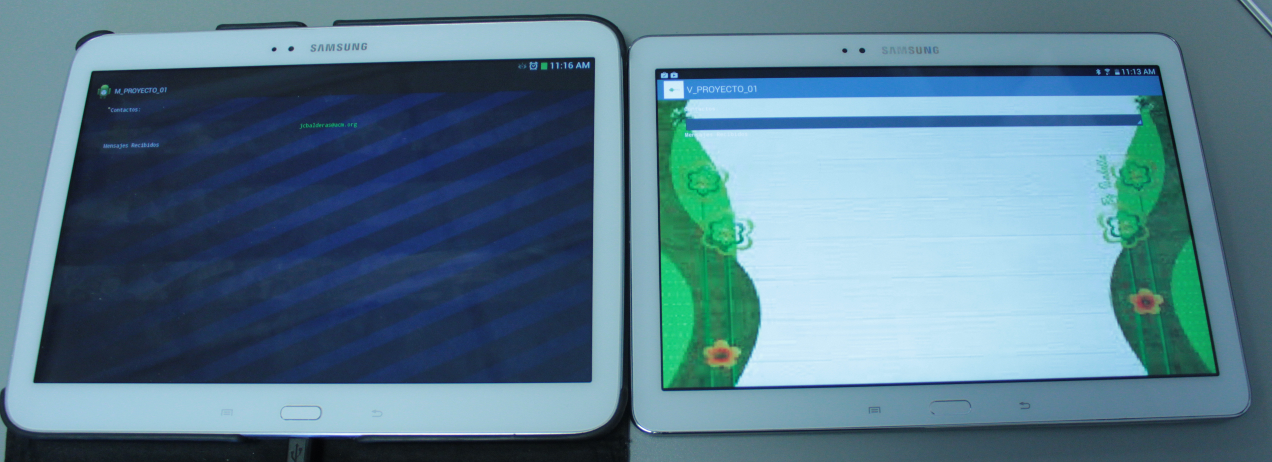
\includegraphics[scale=0.23]{Pirata01}
\end{center}
\end{frame}


\begin{frame}
\frametitle{Plagio}
\begin{columns}[c] % The "c" option specifies centered vertical alignment while the "t" option is used for top vertical alignment
\column{.68\textwidth} % Left column and width
\begin{itemize}
\item Reprobación automática a quien copie códigos de Internet y los reporte como suyos, ademas de una nota en su expediente con copia para el consejo de calidad 
\end{itemize}
\column{.28\textwidth} % Left column and width
\begin{center}

\includegraphics[scale=0.27]{tarjeta-roja}
\end{center}
\end{columns}
\begin{center}
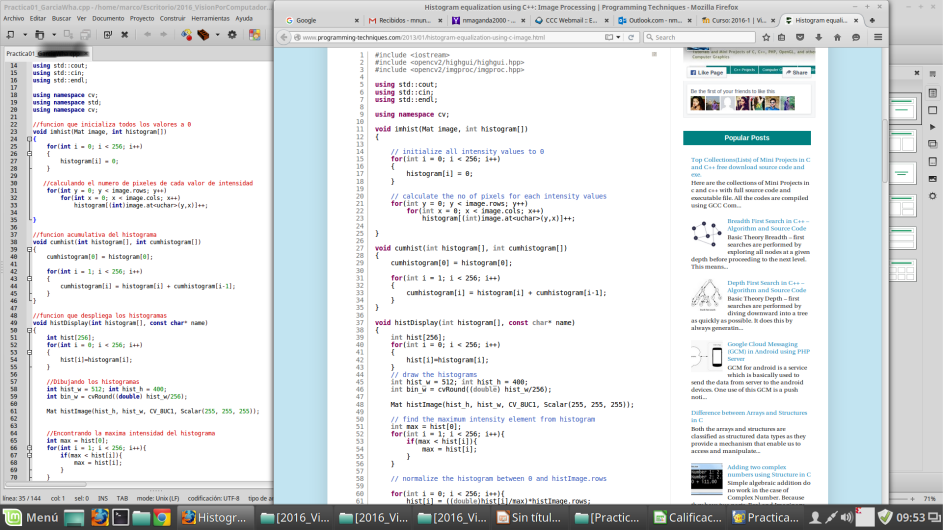
\includegraphics[scale=0.23]{Pifia}
\end{center}
\end{frame}

\begin{frame}
\frametitle{Plagio}
\begin{columns}[c] % The "c" option specifies centered vertical alignment while the "t" option is used for top vertical alignment
\column{.68\textwidth} % Left column and width
\begin{itemize}
\item Reprobación automática a quien copie códigos de Internet y los reporte como suyos, ademas de una nota en su expediente con copia para el consejo de calidad 
\end{itemize}
\column{.28\textwidth} % Left column and width
\begin{center}

\includegraphics[scale=0.27]{tarjeta-roja}
\end{center}
\end{columns}
%\url{https://github.com/naman14/AlgorithmVisualizer-Android}
\href{https://github.com/naman14/AlgorithmVisualizer-Android}{https://github.com/naman14/AlgorithmVisualizer-Android}

\begin{columns}[c] % The "c" option specifies centered vertical alignment while the "t" option is used for top vertical alignment
\column{.44\textwidth} % Left column and width
\begin{center}
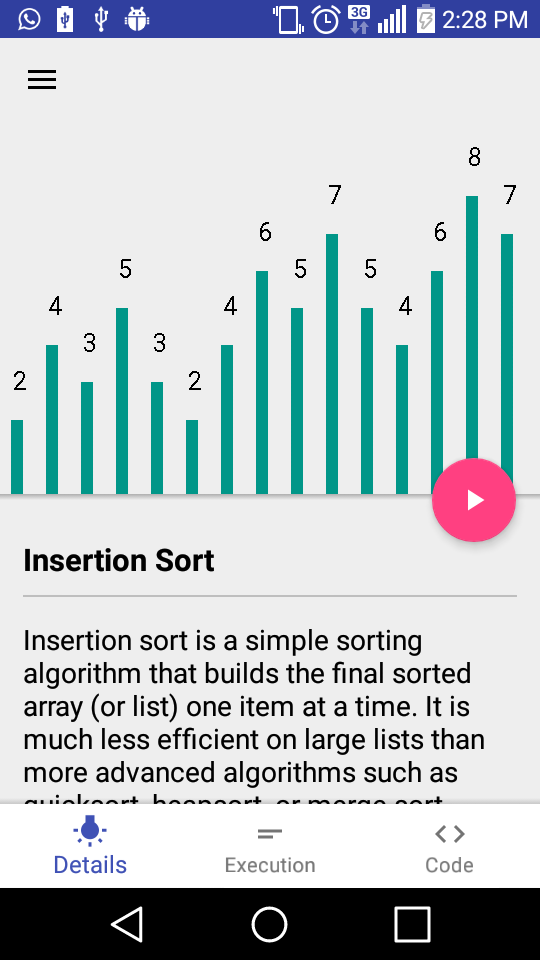
\includegraphics[width=2.3cm]{Piratazo_Orig1}\hspace{0.05cm}
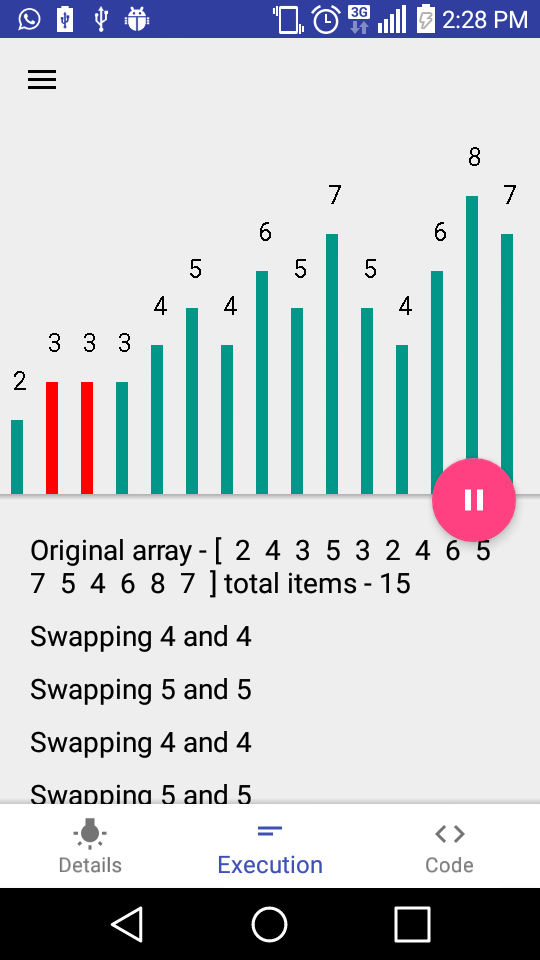
\includegraphics[width=2.3cm]{Piratazo_Orig2}\\
Proyecto Original
\end{center}
\column{.44\textwidth} % Left column and width
\begin{center}
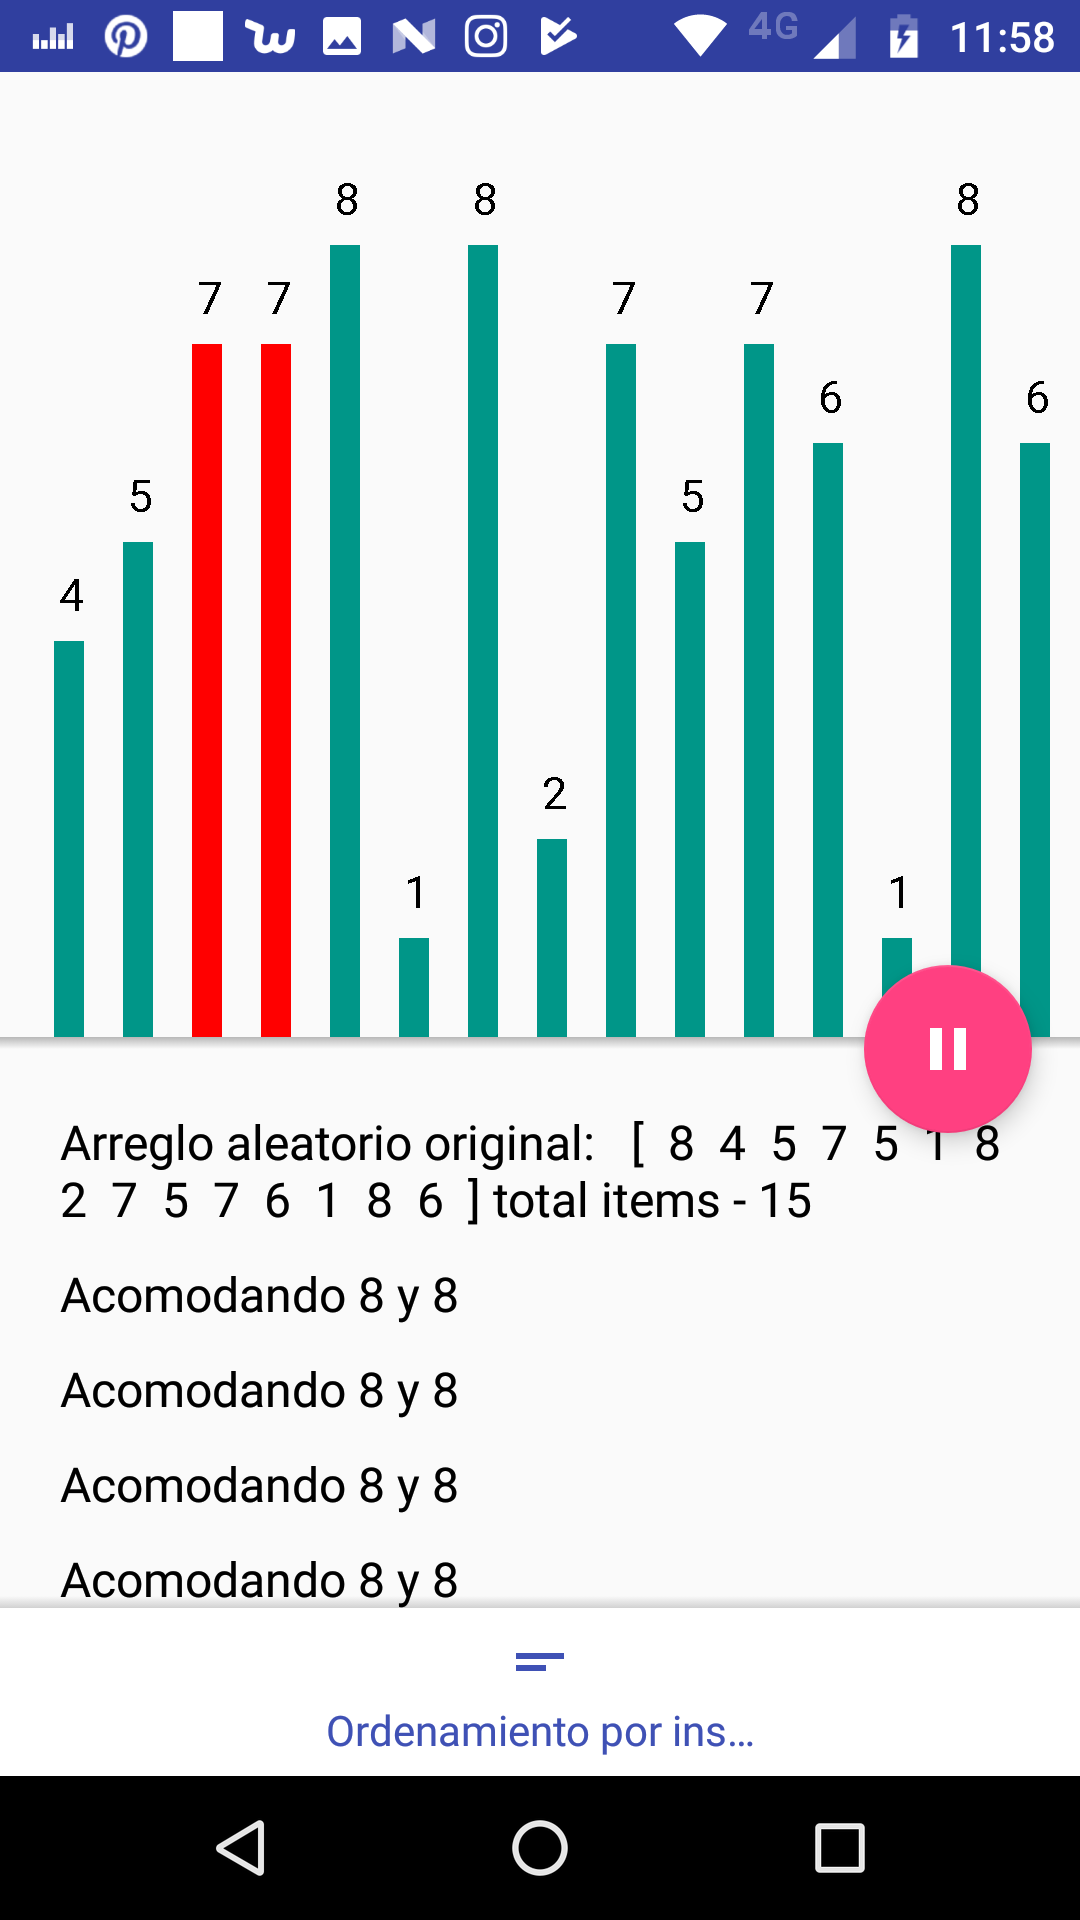
\includegraphics[width=2.3cm]{Piratazo_Oscar1}\hspace{0.05cm}
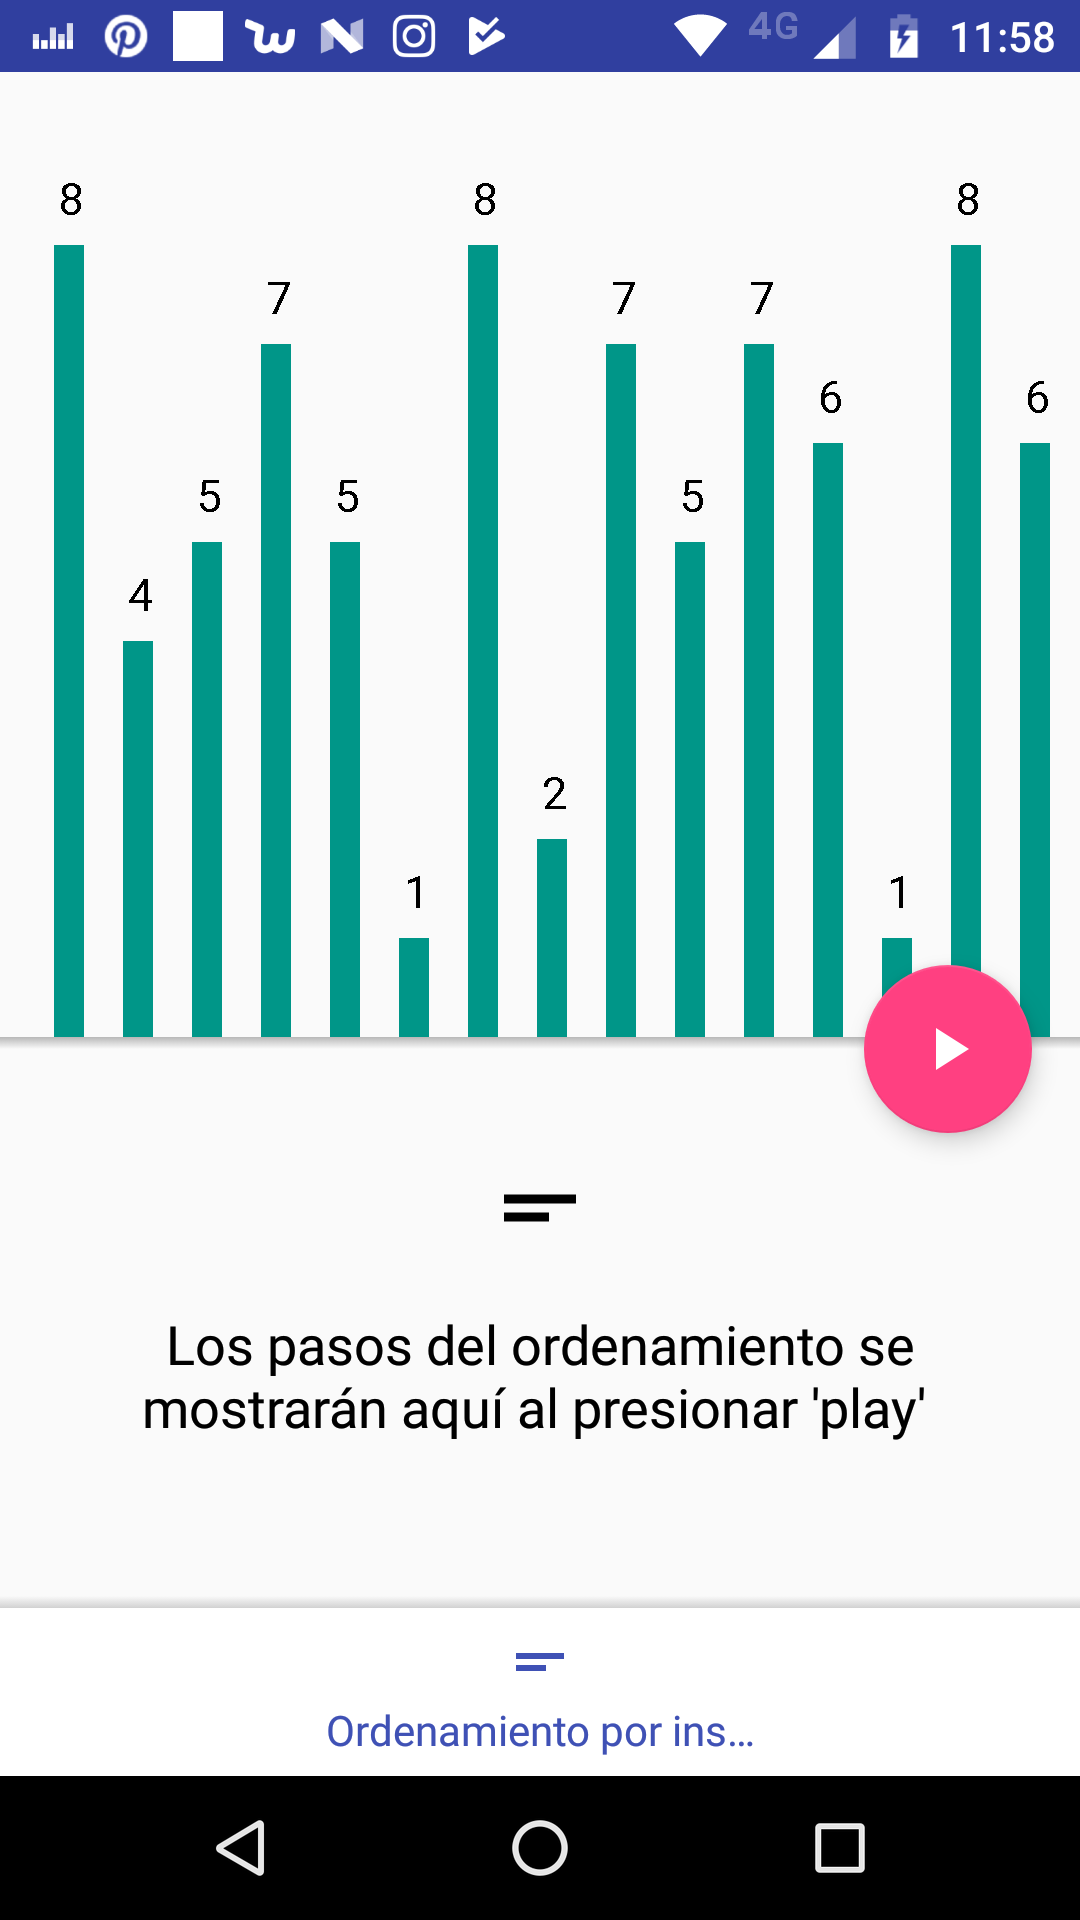
\includegraphics[width=2.3cm]{Piratazo_Oscar2}\\
Proyecto ``clonado''
\end{center}	
\end{columns}
\end{frame}


\begin{frame}
\frametitle{Frase célebre}
``Finalmente son jóvenes que están en la preparatoria y que deben de leer su convocatoria con toda claridad, si no cumplen con los requisitos, si no pueden leer una convocatoria que dice tienes que traer número uno esto, número dos esto, número tres esto, no están listos para ser \textbf{estudiantes de educación superior}, así lo digo con toda claridad''.

Sara Ladrón de Guevara.

Rectora de la Universidad Veracruzana (2013-2017 y 2017-2021).

\end{frame}




\begin{frame}
\frametitle{CONCLUSIÓN}
\begin{center}

\includegraphics[scale=0.31]{UNO}
\end{center}
\end{frame}





\end{document}



